\chapter{Omnidirectional interferometry}\label{ch:omnidirectional}
Parts of this chapter have been submitted as Kagias M, Abis M, Wang Z,
Jefimovs K, Stampanoni M,
\emph{Generalized omnidirectional scattering sensitivity}.

The Talbot-Lau interferometer described in chapter~\ref{ch:review} is one
method of exploiting the self-imaging phenomenon for a periodical wave in
order to transform phase differences into intensity modulations.
An alternative approach has been established on synchrotron
sources~\cite{PhysRevLett.116.093902}, in order to overcome two limitations
of conventional grating interferometry: the limitation of the sensitivity of
the phase and dark-field signals to the direction orthogonal to the grating
lines (equation~\ref{eq:talbot1}); the phase stepping procedure, where
the analyzer grating is scanned across the interference fringes in order to
decode the three characteristic signals
(section~\ref{sec:gi-image-analysis}), which requires multiple exposures and
a precise displacement of the absorption grating \G2 on the order of
hundreds of nanometers.

The setup proposed in~\cite{PhysRevLett.116.093902} relies on the modulation
of a wave front that is periodical in two ways: a unit cell made of
concentric circles introducing a phase shift of $\pi/2$ in the X-rays is
replicated across the field of view
(figure~\ref{fig:omnidirectional-synchrotron}).

\begin{figure}[htb]
    \centering
    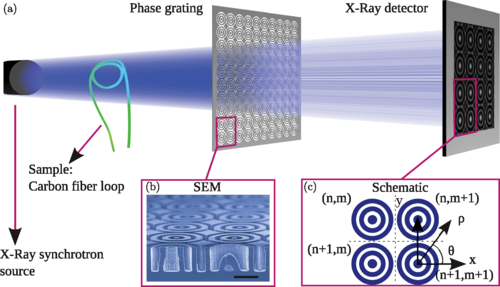
\includegraphics[width=\textwidth]{gfx/omnidirectional/synchrotron-design.png}
    \caption{Experimental setup for a synchrotron omnidirectional grating
    interferometer. The unit cells with concentric circles are shown in the
    \ac{SEM} image and in the recorded interference fringe. Reprinted figure
with permission from Kagias M, Wang Z, Villanueva-Perez P, Jefimovs K,
Stampanoni M, \emph{2D-Omnidirectional Hard-X-Ray Scattering Sensitivity in
a Single Shot}, Phys. Rev. Lett. 116, 9, 093902, 2016. Copyright 2016 by the
American Physical Society.}
    \label{fig:omnidirectional-synchrotron}
\end{figure}

The key feature is the replication of the circular structures 
at the Talbot distances, again according to
equation~\ref{eq:talbot.distance}:
\begin{equation*}
    \Delta_n = n \frac{p_1^2}{2 \lambda} \qquad n \in
    \mathbb{N}.
\end{equation*}
Additional imperfections are introduced by the finite number of periods in
each unit cell, but these are smoothened out as a result of the finite
source size as reported in~\cite{PhysRevLett.116.093902} and this is even
more so in the case of a laboratory source with a compact setup.
This pattern is replicated with a period $P$ of the unit cells themselves,
for which
\begin{equation}
    P = Np_1.
    \label{eq:unit.cell.periop}
\end{equation}

These fringes have to be large enough to be directly resolved at the
detector, as the data from physical detector pixels belonging to the same
unit cell are analyzed together to produce the final image. Analogously to
the phase stepping approach for Talbot-Lau interferometry, each unit cell
records a circular interference fringe that is approximated with a sinusoid

\begin{equation}
    I(x, y) = a_0 + a_1(\theta)\cos\left(\frac{2\pi}{p_1} \sqrt{x^2 +
    y^2}\right),
    \label{eq:omnidirectional.periodical.signal}
\end{equation}

Where $x$ and $y$ are the positions of the pixels with respect to the center
of the unit cell pattern, as identified by the pixel with maximum intensity,
and $\theta = \arctan(y/x)$.

Again similarly to equation~\ref{eq:flat} a comparison between a
\emph{flat} and a \emph{sample} curve with the same shape is required. The
sample will introduce a reduction in the average value $a_0$, related to the
transmission signal; a displacement of the location of the maximum $(x, y)$,
related to the refraction of the X-ray beam; and a reduction in the
visibility of the pattern $a_1$. 

Critically, the dark field signal, or visibility reduction signal, can be
determined as a function of the angle $\phi$ around the circle by calculating the
Fourier transform of the line passing through the center of the unit circle
at the angle $\phi$ and taking the ratio of the $N$-th to the zeroth component

\begin{equation}
    B = \frac{a_{1,s}(\theta = \phi)}{a_{1,f}(\theta =
\phi)}\frac{a_{0,f}}{a_{0,s}}
    \label{eq:dark-field-omnidirectional}
\end{equation}

These are the features of omnidirectional dark-field imaging so far reported
in~\cite{PhysRevLett.116.093902}, our goal is now to export the same
technique from a synchrotron to a conventional X-ray source.
